\documentclass[a4paper]{article}
\usepackage[letterpaper, margin=1in]{geometry} % page format
\usepackage{listings} % this package is for including code
\usepackage{graphicx} % this package is for including figures
\usepackage{amsmath}  % this package is for math and matrices
\usepackage{amsfonts} % this package is for math fonts
\usepackage{tikz} % for drawings
\usepackage{hyperref} % for urls

\title{Homework \LaTeX Template}
\author{Dr. Pablo Rivas}
\date{5/8/16}

\begin{document}
\lstset{language=Python}

\maketitle

\section{Solution to Problem 1.a}
Indeed, problem 1.a assigned based on some paper\cite{HB98} does not really
exist, but it is a good example of how to cite and reference a paper in an
assignment.

\section{Solution to Problem 7.1}
Sometimes you will need to show your mathematical work using equations. Suppose
that you want to explain the way the element of a matrix that is the product of
two others, say $A$ and $B$, at row $i$ and $j$-th column, then you would
probably express that in an equation like this:

\begin{equation}
  c_{ij} = \sum^m_{k=1} a_{ik} b_{kj}
  \label{eq:product}
\end{equation}

You can also reference back to Eq. (\ref{eq:product}) to say that $c_{ij}$ is the
element at any given point in the product matrix $C$.

\subsection{Code}
If you are asked to show your code, you could use a sub-section like this, and
show your code. Here is a way you could do it:

\begin{lstlisting}[frame=single]
import numpy as np

a = [[1, 0], [0, 1]]
b = [[4, 1], [2, 2]]

print np.dot(a, b)

print np.cross(a, b)
\end{lstlisting}

However, note that this code is bad; it is a \textbf{poorly documented} python
script. But if in the last page you will find a good example. Anyway, here is
how you could show the results that your script gives in command line:
\begin{lstlisting}
> python hw1.7.1.py 
[[4 1]
[2 2]]
[1 -2]
\end{lstlisting}
and there it is, the magic of Python and numpy.

\section{Problem 9.1}
Let us also use a sample table. As shown in Table \ref{tbl:aTable} I have some
basketball teams I like. And they can be represented in a floating table.

\begin{table}[h]
 \caption{Some of my favorite teams}
 \label{tbl:aTable}
 \begin{center}
  \begin{tabular}{lccccccr}
    \hline \hline
    Team   & P & W & D & L & F  & A & Score \\
    \hline
    Lakers & 6 & 4 & 0 & 2 & 10 & 5 & 12  \\
    Heat   & 6 & 3 & 0 & 3 &  8 & 9 &  9  \\
    Knicks & 6 & 2 & 1 & 3 &  7 & 8 &  7  \\
    Spurs  & 6 & 2 & 1 & 3 &  5 & 8 &  7  \\
    \hline \hline
  \end{tabular}
 \end{center}
\end{table}

\section{Problem A.1}
Finally lets include a figure produced by some python and matplotlib. The
following python code down below produced Figure \ref{fig:plot}. 

\begin{figure}[h]
  \begin{center}
    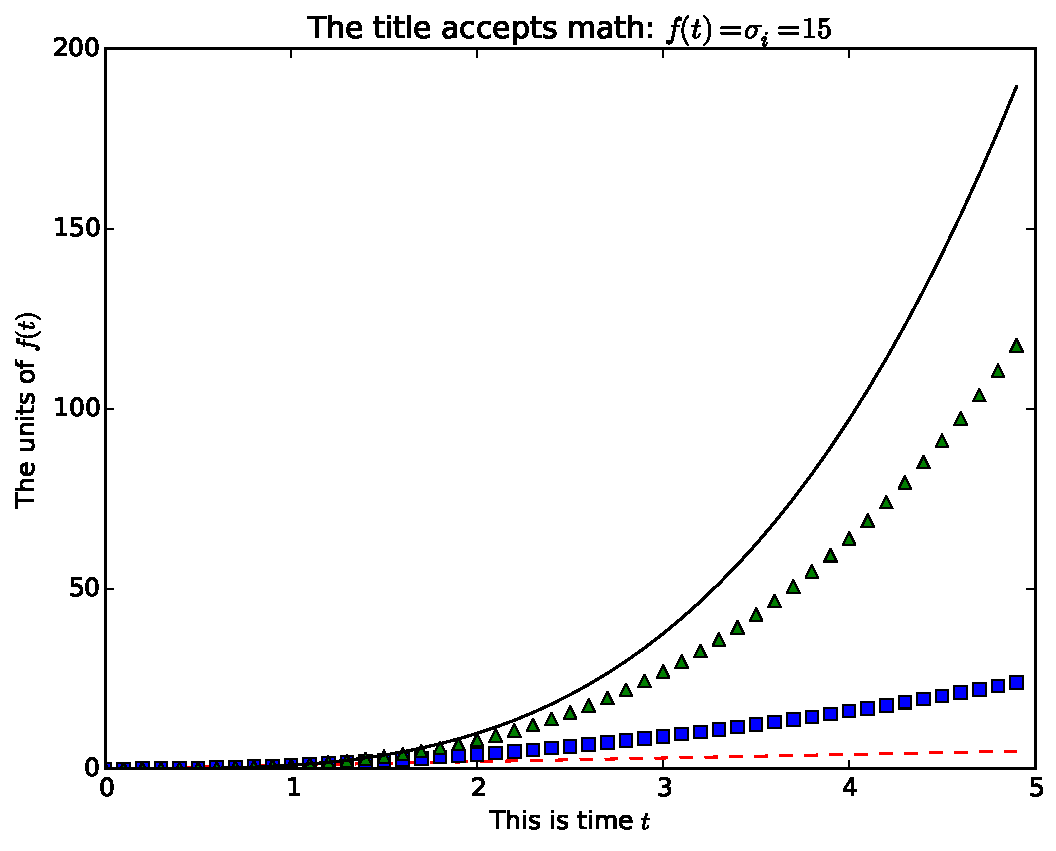
\includegraphics[width=0.75\textwidth]{hwplot.pdf}
  \end{center}
  \caption{The derivative of $f(x)=1-x^2$ at $x=.5$ converging to $-1$ as
  $h\to0$, would be a good example of a good figure caption.}
  \label{fig:plot}
\end{figure}

The name of the file is {\tt hw0.plotme.py} and this should be considered as a
model of a well-documented python program. All your files should have the same
header format as in this file. That is, each python program must have a block
comment at the top which gives the name of the file, the student's name, the
assignment, the date, the version, and a comment about what is contained in the
file. Be concise but precise in your comments. Look at the example that
produced the figure previously mentioned:

\lstinputlisting[language=Python,frame=single]{hw0.plotme.py}

\section{Conclusions}
Feel free to modify this template to suit the needs of what you need to report
in your assignments for this class. If you detect a typo or any other error,
please report it to me. 

\footnotesize
\begin{thebibliography}{99}

  \bibitem{HB98} Huynen, M.~A. and Bork, P. 1998. Measuring genome evolution.
    \emph{Proceedings of the National Academy of Sciences USA} 95:5849--5856.

\end{thebibliography}

\end{document}
